\section{Literature review} \label{sec:litreview}
%Lit. review (actually previous attempts)
%VGG16
%Dahl
%batch norm
%concatenation
%Zhang
%dilation
%classification
 
In recent years, Convolutional neural networks (CNN) have become the standards in image
classification \cite{Krizhevsky}. Using a CNN for image colorization is a trend that has emerged only in the past year in the machine learning community. Research from \cite{Dahl}, \cite{Zhang}
and \cite{Cheng} have shown promising results using CNN, however they all use very different
architectures. One of the problems of using a CNN for image colorization is going back from global features to a mapping of these features in the detailed image space. The use of max-pooling in CNN's makes the network invariant to spatial transformations. However a lot of the spatial information is lost when the final layer of a convential CNN is reached, which is disadvantageous for a classification and localization task. Different techniques have been proposed to regain a local mappping of the features in the final part of the pipeline of the network. Another big variation lies in the loss function of the research mentioned previously. \cite{Dahl}, \cite{Zhang} both use pretrained network's for the front such as VGG16 \cite{Simonyan}, however \cite{cheng}
completely trains the front-end module of the network from scratch. This offers more flexibility with network architecture, however a lot more computational power is required. In
this section a short summary of the related work on image colorization using CNN is shown. In addition the paper by \cite{Simonyan} on VGG16 is explained.

\subsection{Dahl}
The work in this paper is very much an extension to the work of \cite{Dahl}. \cite{Dahl} first converts an RGB image to the YUV colorspace. One of the advantages of the YUV colorspace is that the greyscale values can be used as the Y value. The result of this is that the output of the network, the U and V channels, can be concatenated with the input of the network, resulting in a colorized image. Thus less information needs to be generated by the network. Dahl uses the pretrained VGG16 which already has a big variety of feature extraction. The network was trained on the ImageNet LSVRC 2012 Training Set. Regaining the spatial information from the global features in the bottleneck of the network was done with the use of partial hypercolumns, also called a residual autoencoder \cite{hariharan2015hypercolumns}. The image is upscaled by a factor two after each convolutional layer in the output pipeline of the network. After each upscale operation the feature maps are concatenated with the corresponding feature maps in the input pipeline to regain spatial information as can be seen in \ref{fig:dahlnetwork}. Dahl uses a gaussian blur over the target output of the image, resulting in better guidance of learning. Batch Normalization was applied after every convolutional layer in the input pipeline of the network. Dahls used 3x3 convolutional kernels and ReLu activation functions. The loss function consisted of applying least squares on the euclidian distance between the target pixel values and the output of the network. One of the problems encountered by Dahl was that of color averaging. For classes which have a large variety of color probabilities the network chooses the mean of these colors. For example, cars can have a large variety of colors. The network of Dahl will colorize these cars with the mean of all these colors, so in most cases cars will be colored sepia. Dahl proposes to use generative adversarial networks \cite{Radford}, to counter the color averaging problem. Another method to tackle this problem are variational Auto-encoders, altering a direct copy of the output, (variational) auto encoders are described by \cite{Gregor}, \cite{Kingma} and \cite{GoodfellowBOOK}. 

\begin{figure}
\centering
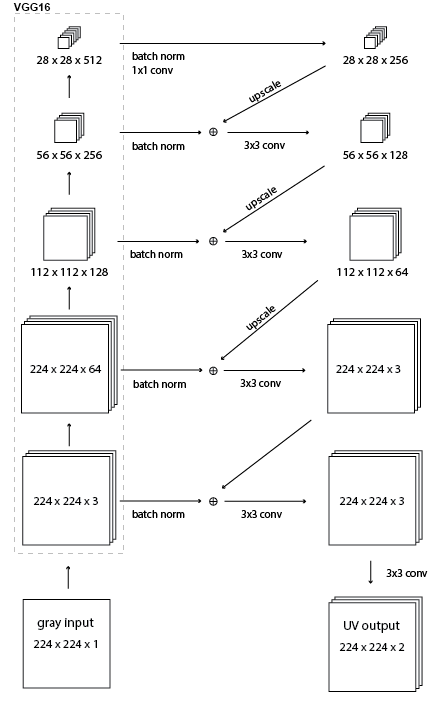
\includegraphics[width=0.5\linewidth]{Dahl_Architecture.png}
\caption{Network used by Dahl \cite{Dahl}}
\label{fig:dahlnetwork}
\end{figure}

\subsection{Zhang et. al}
Very promising results where obtained by Zang et al \cite{Zhang}. Zhang et al propose a fully
automatic approach that produces vibrant and realistic colorizations. Again VGG16 was used for feature extraction. Some modifications where made on the VGG16 architecture. The max-pooling operation is replaced by stride in the incoming convolutional layers, resulting in less loss of spatial information. Also in the output pipeline of the network, use is made of dilated convolutions \cite{yu2015multi}, creating an exponential increasing depth of field with the same number of convolutions as conventional convolutional kernels. In addition the problem was posed as a classification problem, where each output pixel is classified as a certain color. Posing the problem as a classification problem creates the opportunity of implementing class-rebalancing. Categorical cross-entropy was applied on the final softmax output layer of the network. The final loss consisted of the categorical cross-entropy loss multiplied with a value funcion based on the probability of the target color. Colors which are common in the dataset get a low loss, and colors which are rare in the dataset get a high loss, causing the network the 'steer' towards more vibrant colors instead of sepia. 




\subsection{Cheng et al}

\subsection{VGG16}




More literature about convolutional neural networks can be found in \cite{GoodfellowBOOK}. 


%The biggest problem with the machine learning approach to automatic colorization until now, is the case where an object does not have a characteristic color, such as a car or clothing. To solve this problem it is proposed to use generative adversarial networks, to influence the discriminator to be able to generate the right colors where there could be multiple solutions. Generative adversarial networks is described by \cite{Goodfellow} and \cite{Radford}.
%
%The work in this paper is very much an extension to the work of \cite{Dahl}. \cite{Dahl} first converts an RGB image to the YUV colorspace. One of the advantages of the YUV colorspace is that the greyscale values can be used as the Y value. The result of this is that the output of the network, the U and V channels can be concatenated with the input of the network, resulting in a colorized image.

VGG16




Dahl
batch norm
concatenation




Zhang
dilation
classification









The networks described here all use batch normalization layers, this type of layer is first described in \cite{ioffe2015batch}. During training of deep networks the combination of weights and biases can make the nonlinearities to act in the saturated regime causing problems with vanishing gradient. To overcome this the weights need to be initialized carefully and small learning rates are used resulting in slow convergence. Normalizing the output of intermediate layers with respect to each batch that is propagated through the network, makes each subpart of the network less sensitive to the weights and biases of the other parts of the network. This results in faster training due to increased learning rates, the weights initialization can be done less carefully and reduces the need of regularization \cite{ioffe2015batch}.


